\documentclass[prodmode,acmtist]{acmsmall}
\pagenumbering{arabic}

\usepackage{booktabs}
\usepackage{multirow}
%\usepackage{graphix}
\usepackage{lscape}

\usepackage{amssymb}
\usepackage{amsmath}
\usepackage{balance}  % to better equalize the last page
\usepackage{graphicx} % for EPS, load graphicx instead
\usepackage{times}    % comment if you want LaTeX's default font
\usepackage{url}      % llt: nicely formatted URLs
\usepackage[lofdepth,lotdepth]{subfig}
%\usepackage[pdftex]{hyperref}
\usepackage{multirow}
\usepackage{bbm}
\usepackage{pseudocode}
\usepackage{color}
%\usepackage{cite}
%\usepackage{algorithmic}
%\usepackage{algorithm}
%\usepackage[noend]{algpseudocode}
%\usepackage{algorithm}
\usepackage{algpseudocode}
\usepackage[linesnumbered,boxed,ruled]{algorithm2e}

%\newcommand{\modf3}[1]{\textcolor{blue}{#1}}

\newcommand{\TheName}{\mbox{\emph{Daehr}}}
\newcommand{\modif}[1]{{#1}}
\newcommand{\appd}[1]{\textcolor{red}{#1}}


\begin{document}
\title{\TheName{}: a Discriminant Analysis Framework for Electronic Health Record Data  with its Application to Early Detection of Mental Health Disorders}

\author{
HAOYI XIONG
\affil{University of Virginia}
JINGHE ZHANG
\affil{University of Virginia}
YU HUANG
\affil{University of Virginia}
KEVIN LEACH
\affil{University of Virginia}
LAURA E. BARNES
\affil{University of Virginia}
}

%\IEEEcompsoctitleabstractindextext{
\begin{abstract}
Electronic Health Records (EHR) containing a massive number of patient diagnosis records have been used to predict patients' future or potential diseases according to their past diagnoses.
While many data mining tools have been adopted for EHR-based disease early detection, Linear Discriminant Analysis (LDA) is one of the most commonly used statistical methods.
However, it is difficult to train an accurate LDA model to detect specific diseases early when too few patients are known to have the target disease and the EHR data are manually coded with noise.  In such cases, the covariance matrices used in LDA are usually singular and estimated with a large variance.
 
This paper presents \TheName{}, an extending LDA framework using Electronic Health Records, to address these issues.
Beyond existing LDA analyzers, we propose \TheName{} to 1) eliminate the data noise caused by the manual encoding of EHR data, and 2) lower the decision risk of LDA modeld with finely-estimated parameters when only a few patients' EHR are given for training.
To achieve these two goals, we designed an iterative algorithm to improve the covariance matrix estimation with embedded data-noise/decision-risk reduction for LDA.
We evaluated \TheName{} extensively using a large-scale real-world EHR dataset, CHSN.
Specifically, our experiments compared the performance of LDA to three baselines (i.e., LDA and its derivatives) in terms of identifying college students at high risk for mental health disorders from 23 US universities.
Experimental results show \TheName{} significantly outperforms the three baselines by achieving 1.4\%--19.4\% higher accuracy, and a 7.5\%--43.5\% higher F1-score.


\end{abstract}

\category{J.3}{Applied computing}{Health care information systems}

\terms{Human Factors, Algorithms, Performance}

\keywords{predictive models, early detection, anxiety/depression, temporal order, electronic health data}



%\begin{keywords}
%predictive models, early detection, anxiety/depression, temporal order, electronic health data
%\end{keywords}
%}
\maketitle
%\IEEEpeerreviewmaketitle

% For peer review papers, you can put extra information on the cover
% page as needed:
% \ifCLASSOPTIONpeerreview
% \begin{center} \bfseries EDICS Category: 3-BBND \end{center}
% \fi
%
% For peerreview papers, this IEEEtran command inserts a page break and
% creates the second title. It will be ignored for other modes.
%\IEEEpeerreviewmaketitle

\section{Introduction}

With the rapid development of medical big data, forecasting future or potential diseases based on patients' past medical records has emerged as a promising approach towards preventing high-risk diseases.
Rather than individualizing patients (e.g., screening or counseling), a medical informatics system can predict each patient's potential diseases using his or her past diagnoses as well as diagnoses collected from many other patients.
In this way, the medical system can identify high-risk patients from a large corpus of patients with low cost.
These high-risk patients can then receive targeted care to employ disease prevention techniques in advance.
Naturally, the accuracy of such early detection is crucial to improving the efficiency of high-risk patient identification and disease prevention.


In this paper, we present \TheName{}---an extended linear discriminant analysis (LDA)~\cite{fisher1936use,mclachlan2004discriminant} framework for early detection of diseases using Electronic Health Records (EHR), which can improve the prediction accuracy of the standard LDA model by reducing the noise in EHR data and regularizing the estimated covariance matrices.
We first discuss the motivations and background of this research, then we formulate a new research problem based on our observations and assumptions.
We elaborate the technical challenges of the proposed research.
Finally, we summarize our technical contributions.
 

\subsection{Motivations and Backgrounds}

To predict patients' potential diseases according to their past medical records, a variety of predictive models utilizing heterogeneous medical data have been studied~\cite{soni2011predictive,palaniappan2008intelligent,kumari2011comparative}.
For example,  chest imaging has been used for early detection of chest cancer, questionnaire-based assessment (e.g., PHQ-9~\cite{kroenke2002phq}) data for predicting mental health disorders, and screening data for predicting heart disease~\cite{d2001validation}.
Among these medical data, Electronic Health Records (EHR) consisting of the diagnosis records from patients' visits are used as a general purpose data source that enables early detection of diseases based on the previous diagnoses at a massive scale.
Further more, this data is more accessible to clinicians and researchers, and holds comprehensive information of patients' medical history especially within the primary care setting.
Thus, EHR data provides a promising opportunity for  early detection of diseases due to its generality, accessibility and standardized use and features.
 

As shown in Fig.~\ref{fig:exp-ehr}, a patient's EHR data includes all his/her past diagnosis and treatment records, where the diagnosis record includes a sequence of visits, and each visit consists of multiple diagnoses.
Note that all diagnoses are recorded using ICD-9 codes~\cite{dubberke2006icd}, where each evidence of diagnosis corresponds to a specific ICD-9 code.
With diagnosis records in the EHR data, several methods~\cite{personalized2015,amarasingham2010automated,pittman2004integrated,jensen2012mining} have been studied to predict the disease of patients.
Given a disease as the prediction target (e.g., anxiety/depression) as well as the EHR data of a large population with or without the target disease, most existing methods first represent each given patient's EHR data using a set of features, and then train a predictive model using features and labels (if each patient is diagnosed with the targeted disease) in a supervised manner.
Further, given each new patient's EHR data, these models predict if the given patient will develop the targeted disease in near future using the trained predictive model.
 

\begin{figure}
\centering
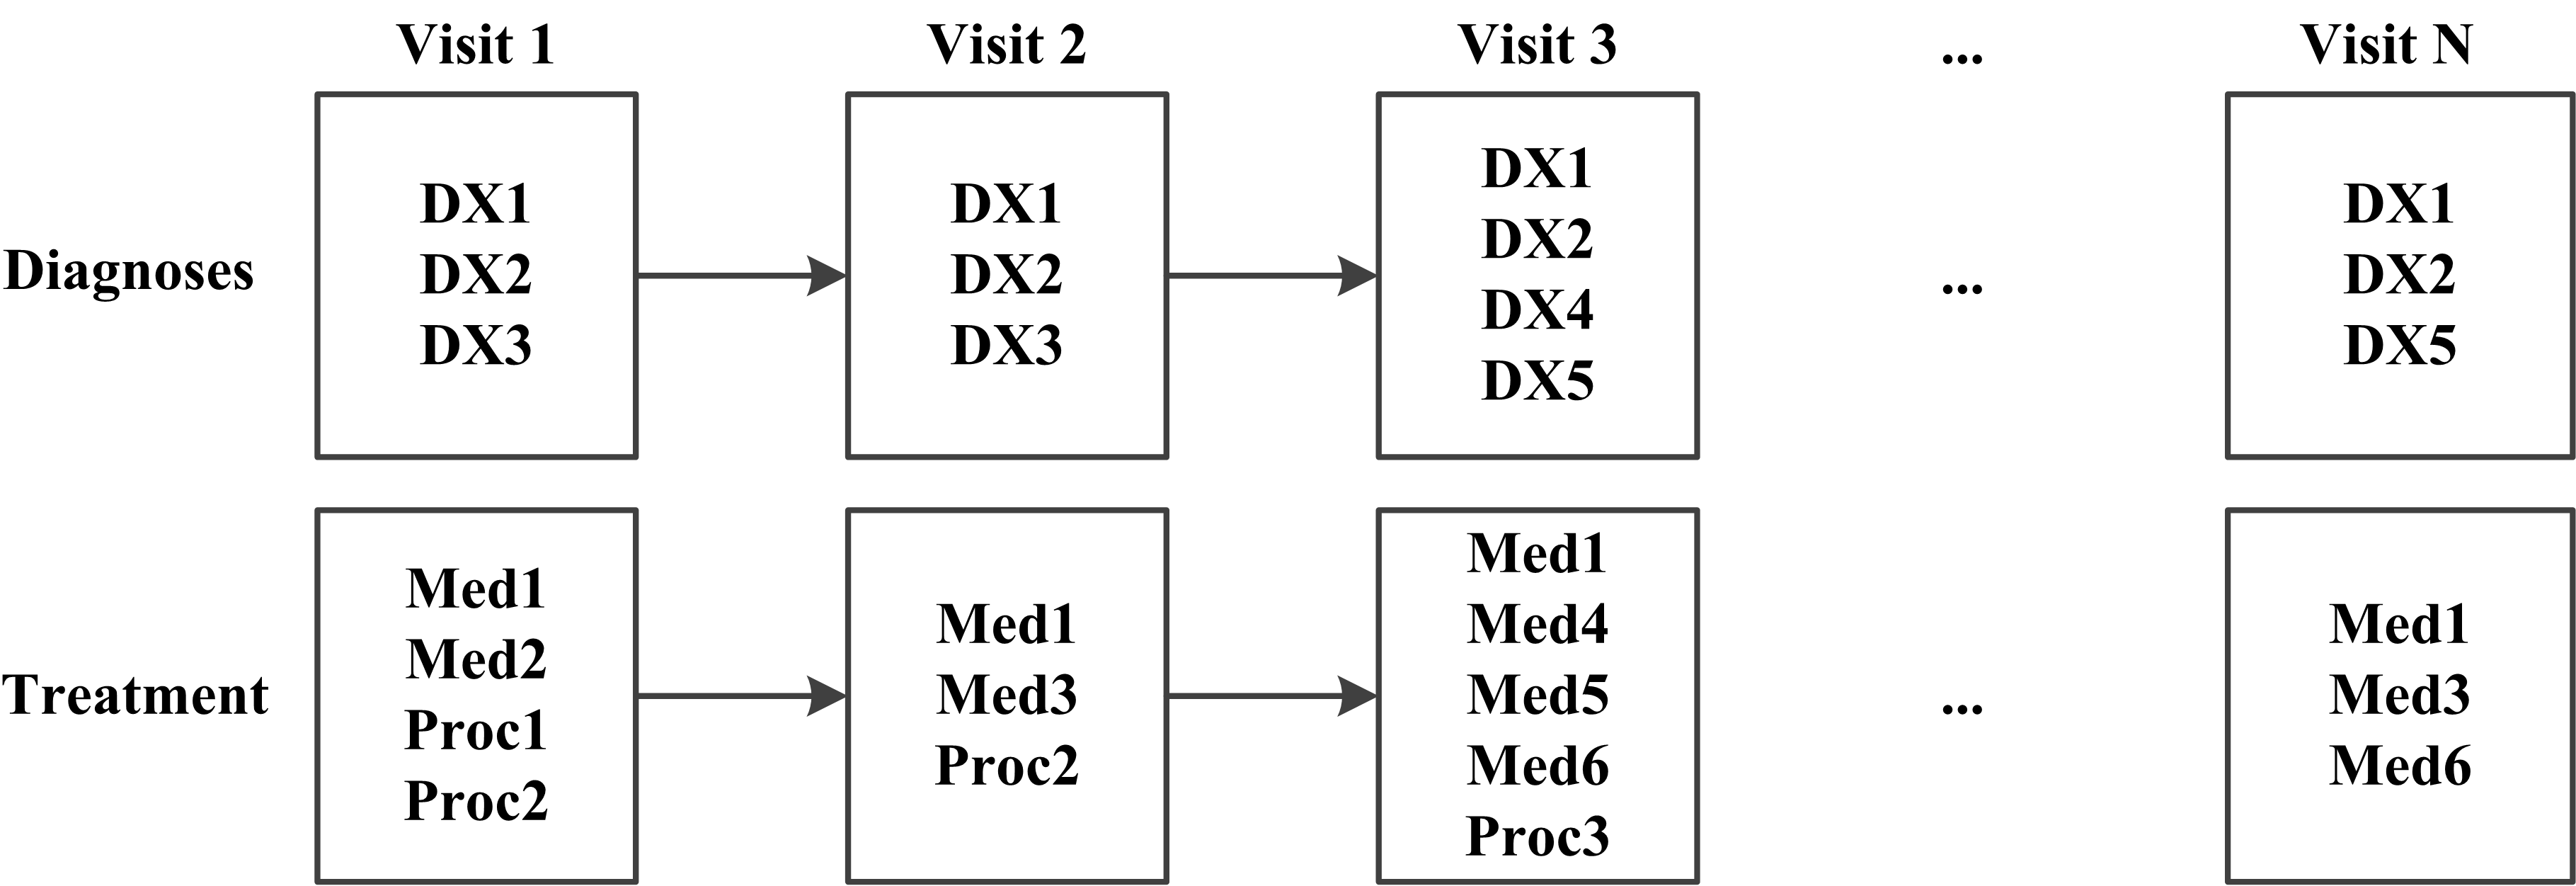
\includegraphics[width=0.88\textwidth]{./img/Patient.png}
\caption{An Example of a Patient's EHR Data}
\label{fig:exp-ehr}
\end{figure}


\textbf{EHR Data Representation for Early Detection.} In terms of representing EHR data, existing approaches include using diagnosis-frequencies~\cite{sun2012supervised,7091853,personalized2015}, pairwise diagnosis transitions~\cite{zhang_mseq_2015,jensen2001mining}, graph representations of diagnosis sequences~\cite{liu_temporal_2015}, and so on.
Among these approaches, the diagnosis-frequency is a common way to represent EHR data.
Given each patient's EHR data, which consists of the patient's demographic information and a sequence of past visits, existing methods first retrieve the diagnosis codes recorded during each visit.
Next, the frequency of each diagnosis appearing in all past visits are counted, followed by further transformation on the frequency of each diagnosis into a vector of frequencies (e.g., $\langle 1, 0, \dots, 3\rangle$, where 0 means the second diagnosis does not exist in all past visits).
In this way, each patient having different number of visits and each visit consisting of multiple diagnoses is represented as a fixed-length data vector, which can be handled by common machine learning algorithms.
 

Note that the diagnosis-frequency representation of EHR data is usually with ultra-high dimensions; for example, there are more than 15,000 ICD-9 codes in EHR scheme, thus the diagnosis-frequency vector using raw ICD-9 codes contains thousands of dimensions.
To reduce the dimensinality, clinical professionals may suggest using clustered code set, where each ICD-9 code can map to  one of the 295 clustered codes.
Thus, each raw diagnosis-frequency vector can be compressed to a vector of around 200 dimensions using clustered codes.
 

\textbf{Supervised Learning for Early Detection.} Given an EHR database and a target disease for early detection, existing methods first select patients both with and without the disease, then use an appropriate representation of their EHR data to form a training set.
To train an accurate predictive model with the training set, many machine learning methods such as Support Vector Machine (SVM), Random Forest (RF), Bayesian Network, Gaussian Process and Linear Discriminant Analysis (LDA) have been adopted~\cite{sun2012supervised,7091853,personalized2015,zhang_mseq_2015,jensen2001mining,liu_temporal_2015,cazzanti_local_2007}.
Among these machine learning methods, LDA is frequently used as one of the common performance benchmarks in a series of studies~\cite{cazzanti_local_2007,zhang_mseq_2015,kalina2013selecting,karlsson2014handling,wang2014clinical}, because it effectively reduces dimensionality.
For example, when using diagnosis-frequency vector as the representation of EHR data, a LDA model learns a linear combination of diagnoses (from the all diagnoses) that can optimally separate patients into the two groups (i.e., with/without the disease).
Then LDA predicts whether new patients will develop the targeted disease by separating their vectors into the two groups using the linear combination.
 

Like many other statistical learning models, the accuracy of a LDA model can be improved, when more samples are given for training.
This is because the decision risk of a LDA model is inherited from the variance of its training samples, while \emph{increasing the sample size lowers the sample variance}~\cite{hsu1947complete,qiao2008effective}.
In contrast, when there are few training samples, the model cannot produce any valid prediction results.
Because LDA needs to use the \emph{inverse of the covariance matrices} to make prediction.
In such case the covariance matrices estimated in LDA are singular or namely \emph{non-invertible}~\cite{huang2002solving,gao2006direct}.
 

We are motivated to enhance the supervised learning methods building upon EHR data so as to improve the prediction accuracy for early detection of diseases.
Specifically, we study the LDA model using the diagnosis-frequency features, because of the relevance of such settings in clinical practices.
 

\subsection{Research Assumptions and Objectives}

Our research is based on following two  observations and two assumptions about EHR data and early detection settings:

\textbf{Observation 1.  EHR Encoding Variation -- }  In terms of encoding EHR data, the diagnosis records are usually inputted manually by clinicians without a unified encoding scheme.
Our previous work~\cite{alicia2015evaluating} finds that, for a single patient, there may be a higher number of diagnosis records for one disease than the number of times that the disease as been diagnosed.
For example, consider three clinicians  Ann,  Bob, and Carl, all working in the same  clinic.
A single patient has been  diagnosed with \emph{upper respiratory infection} (ICD-9 code:  465.9).
Ann may leave only the record of code 465.9 for the first visit  in which the disease is diagnosed.
However,  Bob may leave the  record in the first visit as well as all of the patient's  returning visits to receive  screening or treatment  for  upper respiratory infection.
Carl may leave a record in the first visit and in some of the returning visits at his discretion.


%\emph{three clinicians--Ann, Bob and Carl are working in the same clinics. Given a patient has been diagnosed with upper respiratory infection (ICD-9 code: 465.9), Ann may only leave the record  of code 465.9 in the first visit when the disease is diagnosed. However Bob may leave the record in the first visit as well as all his/her returning visits to receive screening/treatment for upper respiratory infection; while Carl may leave in the first visit and some of the returning visits that he feels necessary.} 

\textbf{\em Assumption I.  Non-negative Noise in Diagnosis-Frequency Vector Data -- } Based upon the first observation, we assume that each diagnosis is recorded at least one time in the EHR and that the number of records might differ due to clinician encoding style (i.e., \emph{frequency of record $\geq$ frequency of diagnosis} for each specific disease).
We further assume the encoding variation of EHR data may cause certain unknown \emph{non-negative data noise} in the diagnosis-frequency vectors.
 

\textbf{Observation 2.  Limited Positive Training Samples -- } We find that the total number of patients with a specific disease (\emph{positive samples}) might be too few to train a predictive model for early detection of the disease.
For example, consider a historically black college that wants to identify the high-risk students in terms of mental health disorders using all students' EHR data in the college clinics.
The clinics first separate all students in to two groups (i.e., with/without mental health disorders diagnosed).
Then it selects a subset of students from each group as training samples.
However, psychiatric clinics are typically underutilized by African American~\cite{thompson2004african}, and thus the available training samples that include at least one type of mental health disorders are two few (e.g., 100-500 students) in the school.


%\emph{a historically black college wants to identify the risk students in terms of mental health disorder using all students' EHR installed in the college clinics. The clinics first sorts all students to two groups (i.e., with/without mental disorder diagnosed), then from each group it selects a subset of students as training samples. However, due to the low utilization rate of psyclinics by African American, the available training samples with at least one type of mental disorders (e.g., depression, anxiety, mood and personality disorders) are so few (e.g., 100$-$500 students) in their school.} 

\textbf{\em Assumption II.  Decision Risk of LDA Model for Early Detection of Diseases -- } Considering the dimension $p$ of diagnosis-frequency vectors (e.g., $p\geq 200$ using clustered code set), we assume that the size of positive samples for LDA training is relatively small i.e., $0<n\lll 2^p$, where $n$ refers to the number of positive training samples.
When $0<n<p$, the trained LDA model cannot produce any valid prediction results, since the estimated covariance matrix is singular/non-invertible; when $p\leq n\lll 2^p$ the trained LDA model might be able to produce a valid prediction, but with large decision risk inherited from the variance of small training samples.
 

With above two assumptions in mind, our work attempts to reduce the effect of noise while lowering the decision risk of the LDA model for early detection of diseases.
Specifically we use mental health disorders as the ``target disease'' in evaluation and experiment design, with respect to  {\em Assumption II}.


\subsection{Technical Issues and Contributions} 
In order to improve LDA with respect to the two assumptions, we address the following three technical issues:
%
\begin{enumerate}
\item \textbf{\em Eliminating the data noise in diagnosis-frequency vectors caused by encoding variation -- } Given the frequency-diagnosis vectors for training, LDA first estimates diagnosis-to-diagnosis covariance matrices using sample covariance matrix estimator such as \emph{Intrinsic Estimator} or \emph{Maximized Likelihood Estimator (MLE)}, then builds the predictive models using estimated covariance matrices.
However, our later analysis shows that the non-negative data noise in the vectors might make the estimated covariance matrices more dense than the noise-free (ideal) one.
In this way, we might need a method to \emph{sparsify} the covariance matrices in order to reduce the effect of data noise to LDA.
 

\item \textbf{\em Lowering the decision risk of LDA while guaranteeing non-singularity and positive definiteness of the estimated covariance matrices - } To lower the decision risk associated with LDA, one possible solution is to use the $\ell_1$-penalized estimation of the covariance matrices~\cite{cai2012minimax,xue2012positive}.
However, any modifications (including $\ell_1$-penalty and sparse approximation) to a coavriance matrix might result in loss of its positive definiteness---we cannot use such modified matrix in the statistics model.
We need an algorithm to obtain the $\ell_1$-penalized estimation of the sparsifed covariance matrix while ensuring the estimation is non-singular and positive semidefinite.


\item \textbf{ \em Incorporating the newly-estimated covariance matrices for improving the performance of EHR-based LDA -- } Given the non-singular/positive-definite $\ell_1$-penalized sparse estimations of the  covariance matrices, we might need use them to replace the covariance matrices originally used in LDA.
Thus, we need a generic framework to extend the original LDA through incorporating the aforementioned covariance matrix estimation algorithms.
More important, we must make sure that, compared to LDA, the new framework should provide better overall accuracy and F1-score for early detection of the diseases.
While most existing predictive models consider overall accuracy as the primary performance metrics, F1-score, characterizing both correctness and completeness to identify high-risk patients from large testing samples, is yet another important metrics of our problem.
An early detection framework with higher F1-score usually can identify more high-risk patients with fewer false alarms.
Note that a predictive model with improved overall accuracy is not necessarily to have better F1-score.
Thus, though it might be hard to achieve the two goals together, we need such a framework that can improve both accuracy and F1-score.


\end{enumerate}
%
With the aforementioned research challenges in mind, we make following technical contributions in this study:
%
\begin{itemize}
    \item In this work, we studied the problem of improving the existing Linear Discriminant Analysis (LDA) for early detection of diseases based on our two assumptions.
To the best of our knowledge, this paper is the first work for LDA-based early detection of diseases built upon EHR data, by addressing the issues of encoding variation and low training sample size.


\item In order to address these technical challenges, we proposed \TheName{}---an extending LDA framework.
It takes a novel approach to eliminate the affect of data noise and lower the decision risk of LDA models  through estimating sparse and non-singular diagnosis-to-diagnosis covariance matrices from diagnosis-frequency vectors.
Theoretical analysis shows that, with low computational complexity, the proposed algorithm can approximate the $\ell_1$-penalized near-sparsest estimation of the diagnosis-to-diagnosis covariance matrices with non-singularity and positive semi-definiteness guaranteed, even when a very limited number of diagnosis-frequency vectors are given for LDA training.


\item We evaluated \TheName{} using a real-world dataset CHSN,  which contains more than 300,000 students' EHR records collected from 23 US universities in past three years.
We designed a set of experiments based on CHSN for large-scale early detection of mental disorders.
The experimental results show \TheName{} significantly outperforms three baselines (i.e., LDA and its derivatives) by achieving 3\%--10\% higher prediction accuracy, and 3\%--14\% higher F1-score.


\end{itemize}

The paper is structured as follows: Section~\ref{sec:2} discusses the previous studies that have been done in the data mining approaches to early detection of disease and LDA extensions.
Section~\ref{sec:3} introduces the problem formulation of our study and introduces the \TheName{} framework to solved the problem.
Section~\ref{sec:4} describes two core algorithms used in \TheName{}.
Section~\ref{sec:5} describes the data used in this research, the experimental design, and the experimental results and analyses.
Finally, the summary of this work, future work, and clinical context are discussed in Section~\ref{sec:6}.
 


\section{Related Work}\label{sec:2}

% machine learning in medical area
In this section, we summarize previous studies related to this paper from two aspects: \emph{data mining approaches to early detection of diseases} and \emph{extensions to LDA learning}.

\subsection{Big Data Approaches to Disease Early Detection}

Various analytical methods have been used to study the causes, prevention, progression, and interventions of diseases.
Among these methods, machine learning emerged as a promising technique in the prediction of diseases ~\cite{maroco_data_2011,huang_toward_2014}.
In this section, we will discuss previous work in two areas: \emph{predictive modeling} and \emph{data representation} approaches.


\subsubsection{Predictive Models for Early Detection of Disease} 

Predictive models have become popular in the early detection of diseases, such as breast cancer, type II diabetes and cardiovascular disease~\cite{Lindstrom01032003,riskprediction,zheng_predictive_2015,yoo_data_2011}.
The outcomes of the predictive models are beneficial to both care providers and patients.
Accurate prediction of diseases can assist clinicians in identifying high-risk patients in an early stage, ultimately leading to more timely diagnoses and more focused delivery of effective treatments to those patients.
In essence, the early detection of diseases can be viewed as a classification problem so that well-established classifiers can be used to perform the task.
Among the studies on the early detection of mental disorders, a LASSO logistic regression model has been applied to predict the depression severity to help personalize treatment for high-risk patients~\cite{huang_toward_2014}.
%In this work, the feature vector used for prediction includes gender, ICD-9 codes, disease and drug ingredient terms, and average number of visits. 
%However, the predictive model is more accurate in recognizing low risk-patients and achieves a 90\% specificity, while the sensitivity are 25\% using the information 12 months before the diagnosis and 50\% at the time of diagnosis, respectively~\cite{huang_toward_2014}.
  
\subsubsection{EHR Data Representation for Predictive Models. } 

%Electronic health data is highly accessible in health care institutions and has become a promising data source for public health research.
%However, EHR data is heterogeneous and cannot be readily expressed in a unified vector space.
%Thus, an appropriate representation of those data is critical for further advancements in analytics and modeling.
 
Many data representation approaches have been developed to preserve useful information from the raw EHR data.
Diagnosis-frequency vectors have been proposed~\cite{ng_personalized_2015,huang_toward_2014} to convert sequences of diagnoses with different lengths into fixed-length data vectors.
This approach associates each patient with an intuitive notion of an ``intensity'' of each disease with which a patient has been diagnosed.
Because such vectors can be easily handled by common predictive models without further data representation.
Some novel representation methods have been proposed to characterize the temporal order information in patients' diagnosis sequences using the frequencies of transitions between diagnoses~\cite{zhang_mseq_2015,wang_towards_2012,liu_temporal_2015,gotz_methodology_2014,perer_frequence:_2014,perer_mining_2015}.
Specifically,~\cite{zhang_mseq_2015} intends to project the frequency of transition between each two diagnoses onto a fully-connected graph, while~\cite{liu_temporal_2015} preserves the frequencies of important transitions using sparse graph representation and penalty.
While previous work usually considers the frequency of pairwise transitions between each two diagnoses,~\cite{gotz_methodology_2014,perer_frequence:_2014,perer_mining_2015} consider the frequencies of transitions crossing multiple diagnoses using a hyper-graph.

%In~\cite{wang_framework_2012}, Wang et al. use a spatial-temporal matrix to represent the a sequence of events in which the two dimensions represents the event type and time information, respectively. In~\cite{liu_temporal_2015}, Liu et al. considers events in a patient's EHR is represented by a temporal graph and basis graphs are learned as the features to represent patients. Furthermore, frequent sequence mining has been utilized to uncover the most important event sequences~\cite{}. In~\cite{gotz_methodology_2014}, Gotz combine the episode definition and temporal pattern mining techniques to support the visual exploration of the clinical event patterns with most impact. 

% move to discussion
%To address high dimensional data, FeaFiner~\cite{zhou_feafiner:_2013} uses simultaneous feature grouping and selection. It extracts relevant and non-overlapping feature concepts in a low dimensional space, where the prediction accuracy is improved when applied to predicting Alzheimer’s Disease-related scores~\cite{zhou_feafiner:_2013}. 

\subsection{Extensions to LDA Model}

We introduce several LDA extensions in High Dimension Low Sample Size (HDLSS) settings such as those challenges presented by EHR data .
As discussed above, when LDA works in HDLSS, there exists two major technical issues: 1) LDA requires inverting covariance matrices for classification, but these covariance matrices estimated from small number of samples are usually singular (non-invertible), and 2) large decision risk is inherited from the variance of small samples, through classical LDA training.
To handle the singular (non-invertible) covariance matrix issue, Ye et al.~\cite{ye2004optimization} uses the Pseudo-inverse of the singular covariance matrix, while Direct LDA~\cite{lu2003face,gao2006direct} uses the \emph{simultaneous diagonalization} of covariance matrices, which are non-singular, to replace the original covariance matrices.
On the other hand, several works~\cite{clemmensen2011sparse,qiao2008effective,shao2011sparse} have proposed lowering the decision risk via regularizing the estimated covariance matrices.


\TheName{} is distinct in three ways.
First, compared to other data mining approaches to early detection of diseases (e.g.,~\cite{Lindstrom01032003,riskprediction,zheng_predictive_2015,yoo_data_2011}), \TheName{} is the first work that intends to improve the performance of LDA model by addressing data noise and small positive training sample size issues.
%
%%What are these works?
Second our contribution is complementary with these works in EHR data representation~\cite{wang_towards_2012,wang_framework_2012,liu_temporal_2015} and we can further improve \TheName{} by incorporating advanced EHR data representation methods.
Third, when compared to existing LDA extensions, \TheName{} re-estimates the covariance matrices to (1)  eliminate the effect of data noise to LDA model, (2) lower the decision risk inherited from  small positive training samples, and (3) guarantee the non-singularity of covariance matrices, while~\cite{ye2004optimization,lu2003face,gao2006direct,clemmensen2011sparse,qiao2008effective,shao2011sparse} all focus on regularizing the covariance matrices to enable LDA in a general HDLSS setting.
Thus, the estimation/optimization problems considered in any single one of the previous studies are mathematically different from ours with different objectives and assumptions.



\section{\TheName{} System Model}\label{sec:3}
In this section, we first formulate the research problem of our study; then we propose \TheName{} framework to solve the formulated problem.

\subsection{Problem Formulations}

According to our research assumptions, in this section, we make two definitions and introduce several preliminary studies used in our studies.
Further, we formulate our research problem based on all above definitions and preliminaries.


\textbf{\em Definition I.} \emph{Diagnosis-frequency Vector and Non-negative Noise Vector -- } Given EHR data of $m$ patients (both with and without the targeted disease), we can extract $m$ diagnosis-frequency vectors $X_0,X_1\dots X_{m-1}$.
Each vector e.g., $X_i=<1,0,\dots,3>$ consists of two parts: $\hat{X}_1$ the vector of true diagnosis frequencies (not diagnosis record frequencies) and $E_i$ the non-negative noise vector: 

\begin{equation}
X_i=\hat{X}_1+E_i
\end{equation}

\textbf{\em Preliminary I.
}\emph{Generalized Two-class LDA and Covariance Matrices -- } According to the common implementation of a LDA classifier~\cite{ziegel2003modern}, given $m$  training samples as well as the labels i.e., $(X_0,l_0)\dots (X_{m-1},l_{m-1})$ where $l_i\in\{-1,+1\}$ refers to whether the patient $i$ has been diagnosed with the target disease (i.e., positive sample or negative sample),  a two-class LDA  model first sorts each sample into two groups according to the label, and estimates covariance matrix/mean vector of the two classes, i.e., ($\Sigma_{+}$, $\mu_+$) and ($\Sigma_{-}$,$\mu_-$), using the positive samples and negative samples respectively.
Then generalized two-class LDA determine if a new patient ($X'$) would develop to the targeted disease, using 
%
\begin{equation}
\begin{aligned}
&(X'-\mu_-)^T\Sigma_{-}^{-1}(X'-\mu_-)+ln|\Sigma_-|-\\
&(X'-\mu_+)^T\Sigma_{+}^{-1}(X'-\mu_+)-ln|\Sigma_+|<T,
\end{aligned}
\label{eq:glda}
\end{equation}
where $T$ is an optimal threshold based on the training samples.
However, as illustrated in our observation 2,  when positive sample size is relatively small e.g., for the rare disease in the database,  $Rank(\Sigma_+)<p$,  $\Sigma_{+}$ is singular and $\Sigma_{+}^{-1}$  doesn't exist.
In this case, Equation~\ref{eq:glda} might not work.


Please note that in the rest of paper we name the both $\Sigma_{+}$ and $\Sigma_{-}$  as a \emph{covariance matrix} simply, since they are considered equally in our problem formulation and solution design; in contrast, the covariance matrix may refer to the either $\Sigma_{+}$ or $\Sigma_{-}$.


\textbf{\em Definition II.} \emph{Sample Diagnosis-to-Diagnosis Covariance Matrix Estimation and Disturbance of Non-negative Noise -- } With above settings in mind, we further define $\Sigma$ as the sample diagnosis-to-diagnosis covariance matrix based on noisy data, $\hat{\Sigma}$ as the sample covariance matrix based on ``noisy-free'' vectors, and  $\Delta=\Sigma-\hat{\Sigma}$ as the disturbance of non-negative noise to covariance estimation.

\begin{equation}
\begin{aligned}
\Sigma&=\frac{1}{n}\sum_{i=0}^{n-1} X_iX_i^T
=\frac{1}{n}\sum_{i=0}^{n-1} (\hat{X}_i+E_i)(\hat{X}_i+E_i)^T\\
&=\hat{\Sigma}+\Delta
\end{aligned}
\label{eq:sample-cov}
\end{equation}

As the sample covariance matrix estimation shown in~\ref{eq:sample-cov}, the disturbance should be:

$$\Delta=\frac{1}{n}\sum_{i=0}^{n-1}(2\hat{X}_iE_i^T+E_iE_i^T).$$ 

According to our definition $\hat{X}_i$ and $E_i$ are both non-negative matrices, it is not hard to find that $\Delta=\Sigma-\hat{\Sigma}\geq \textbf{0}$ is a non-negative matrix and $||\Sigma||\geq ||\hat{\Sigma}||$.
Thus, we can roughly conclude that $\hat{\Sigma}$ might be a sparse estimation of $\Sigma$.
 

\textbf{\em Preliminary II.  } \emph{Minimax risk estimation of the covariance matrix in HDLSS settings -- } Previous work~\cite{cai2012minimax,xue2012positive} showed that it is possible to achieve \emph{minimax risk} covariance matrix estimation from a few samples, using the \emph{minimal $\ell_1$-normal estimation} of the original sample covariance matrix.
In this case, in terms of lowering variance of LDA, we can assume that the optimal~\cite{cai2012minimax} covariance matrix $\tilde{\Sigma}$ should be a $\ell_1$-penalized sparse estimation of $\hat{\Sigma}$.


\textbf{Problem Formulation.  } According to above definitions and preliminaries, this paper considers a problem of finding the positive-definite sparse estimation of $\hat{\Sigma}$-the noisy-free diagnosis-to-diagnosis covariance matrices, to improve the performance of LDA for early detection of disease.
Hereby, we define our research problem that, Given $n$ diagnosis-frequency vectors $X_0,X_1\dots X_{n-1}$,  our problem is to estimate $\tilde{\Sigma}$: 

\begin{equation}
\begin{aligned}
\text{min. }|\tilde{\Sigma}|_1 \text{ s.t. }||\tilde{\Sigma}-\hat{\Sigma}||_F^2\leq \epsilon\text{ and }\tilde{\Sigma}\in {\bf }I^+
\end{aligned}
\label{eq:problem}
\end{equation}
where ${\bf }I^+$ refers to the overall set of positive semidefinite matrices. 
Please note that $\hat{\Sigma}$ is not foreknown due to the unknown data noise. 

Intuitively, it is possible to solve the formulated problem through sparsifying and regularizing the sample diagnosis-to-diagnosis covariance matrix $\Sigma$ subject to the positive semidefinite and non-singularity constraint. 


\begin{figure}
\begin{center}
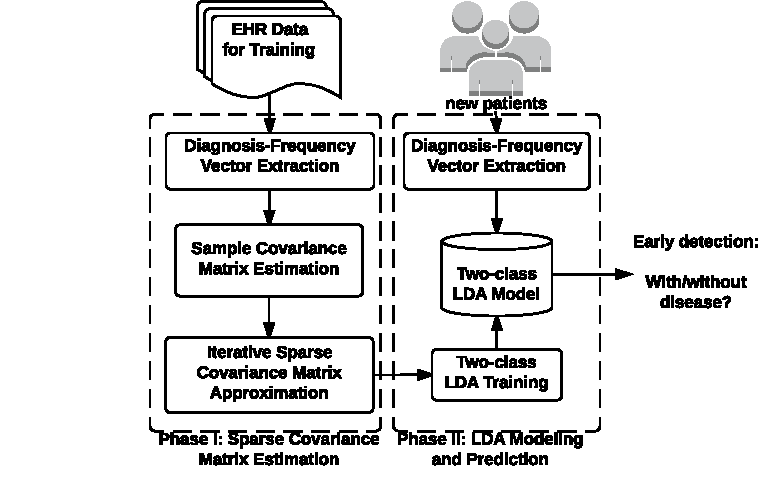
\includegraphics[width=0.98\textwidth]{./img/daehr.pdf}
\end{center}
\caption{\TheName{} Framework}
\end{figure}


\subsection{\TheName{} Framework}
In this section, we introduce the framework design of \TheName{}. 
\TheName{} consists of two phases.  
First, we use the EHR data for training to estimate the covariance matrices used in LDA with respect to our problem formulation. 
Next, we adopt LDA with newly estimated parameters to predict whether the new patient will develop the targeted disease.

\emph{Phase I: Sparse Covariance Matrix Estimation --- } Given the patients' EHR data as a training set, this phase estimates the sparse covariance matrices for two classes of patients with following two steps:
\begin{enumerate}

    \item \textbf{Diagnosis-frequency Vector Extraction and Sample Covariance Matrix Estimation --- } \TheName{} first converts each patient's EHR data to a diagnosis-frequency vector and combines it with his/her label (indicating whether the patient has been diagnosed with the targeted disease).
Specifically, we acquire $(X_0,l_0)\dots (X_{m-1},l_{m-1})$, where $l_i\in\{-1,+1\}$ is the label of the $i^{th}$ patient.
With the vectors corresponding to each of the two classes, \TheName{} then estimates the sample covariance matrices for the two classes $\Sigma_+$ and $\Sigma_-$ using Equation~\ref{eq:sample-cov}.  


    \item \textbf{Iterative Sparse Covariance Matrix Approximation --- } Given sample covariance matrices $\Sigma_+$ and $\Sigma_-$, \TheName{} estimates the positive-definite $\ell_1$-penalized estimation of both $\Sigma_+$ and $\Sigma_-$ using a unified iterative approximation process, where \TheName{} treats $\Sigma_+$ and $\Sigma_-$ equally.
     As shown in Algorithm~\ref{alg:iap}, given an input sample covariance matrix $\Sigma_0=\Sigma_+$ or $\Sigma_-$, the process iteratively approximates to the positive definite $\ell_1$-penalized estimation of $\Sigma_0$ through alternating between two algorithms---\emph{$\ell_1$-penalized Sparse Matrix Estimation} and \emph{Nearest Positive Semidefinite Matrix Approximation} in each iteration.
In Algorithm~\ref{alg:iap}, $\Delta'=\frac{||\Sigma_{t+1}-\Sigma_{t}||_\infty}{||\Sigma_{t}||_\infty}$ and $tol$ is a threshold characterizing the tolerance of convergence.
     Specifically, in each (i.e., the $t^{th}$, $t\geq 0$) iteration, the process obtains an improved result $\Sigma_{t+1}$ using the previous result $\Sigma_{t}$.
     With the result improved each iteration, the algorithm stops only when the predefined convergence is achieved ($\Delta''< tol$) or after iterating $maxit'$ times (i.e., $t>maxit'$).
 

\end{enumerate}
Note that the covariance matrices for the two classes of patients are estimated in this phase through a unified process.
We denote the new covariance matrices as $\Sigma_+^*$ and $\Sigma_-^*$ for the positive and negative classes, respectively.

\begin{algorithm}
\caption{Iterative Approximation Process for Sparse Covariance Matrix Estimation}
\label{alg:iap}
\KwData{$\Sigma_{0}$ --- the sample covariance matrix i.e., $\Sigma_+$ or $\Sigma_-$}
\KwResult{${\Sigma_{t+1}}$ --- the positive definite $\ell_1$-penalized estimation of $\Sigma_0$}
\Begin{
\While{ $\Delta' \geq tol, \text{ or }0\leq t \leq maxit'$  }{
	$\Sigma_{t+\frac{1}{2}}\gets \ell_1$-penalized sparse estimation of $\Sigma_t$\\
    $\Sigma_{t+1}\gets $ the nearest positive semidefinite approximation to  $\Sigma_{t+\frac{1}{2}}$
}
\Return{$\Sigma_{t+1}$}
}
\end{algorithm}


\emph{Phase II: LDA Modelling and Prediction --- } Given the two estimated matrices $\Sigma_+$ and $\Sigma_-$ as well as the training samples, this phase first trains the optimal model for LDA prediction. 
Then, it uses the LDA model for new patient prediction. 
This phase consists of following two steps:
\begin{enumerate}
    \item \textbf{LDA Model Training --- } Given the two estimated covariance matrices $\Sigma_+^*$ and $\Sigma_-^*$ as well as training samples $(X_0,l_0)\dots (X_{m-1},l_{m-1})$, \TheName{} searches for the optimal threshold $T^*$ that can maximally classify the two classes of samples using Equation~\ref{eq:glda}. 
        In this case, \TheName{} uses a LDA model as $(\Sigma_+^*,\mu_+,\Sigma_-^*,\mu_-,T^*)$.
    \item \textbf{LDA-based new Patient Prediction --- } Given a new patient's EHR data, \TheName{} first converts her data to a diagnosis-frequency vector (e.g., $X'$). 
        Combined with the LDA model described as $(\Sigma_+^*,\mu_+,\Sigma_-^*,\mu_-,T^*)$, \TheName{} predicts whether the patient will develop the targeted disease using the criterion in Equation~\ref{eq:glda}.
\end{enumerate}
%

After the above two phases terminate, \TheName{} will have (1) learned a LDA model with advanced covariance matrix estimation, and (2)  adopted the LDA model to enable the early detection of targeted disease. 
Though the architecture of the framework is discussed here, the design of the aforementioned \emph{$\ell_1$-penalized Sparse Matrix Estimation} and \emph{Nearest Positive Semi-Definite Matrix Approximation} algorithms are discussed in following sections.


\section{\TheName{} Core Algorithms}~\label{sec:4}
In this section, we first introduce the two core algorithm used in \TheName{}, then analyze the performance of the proposed algorithms.

\subsection{$\ell_1$-penalized Sparse Matrix Estimation}
Given the covariance matrix estimated in the previous iteration $\Sigma_{t}$, this algorithm estimates $\Sigma_{t+\frac{1}{2}}$ --- the $\ell_1$-penalized sparse estimation of $\Sigma_{t}$, using the Proximal Gradient Descent algorithm~\cite{nesterov2004introductory} with following objective function:   
\begin{equation}
\emph{min. }\frac{1}{2}||\Sigma_{t+\frac{1}{2}}-\Sigma_t||_F^2+\lambda |\Sigma_{t+\frac{1}{2}}|_1,
\label{eq:sparse-imp}
\end{equation}
where $\lambda$ is a Lagrange multiplier~\cite{wu2009karush}. 
When $\lambda\geq 0$, the Eq.~\ref{eq:sparse-imp} is a \emph{convex function with sparse input}, which can be optimally converged using proximal gradient descent~\cite{nesterov2004introductory}. 
Note that $\Sigma_{t+\frac{1}{2}}$ is neither symmetric nor positive semidefinite.



\subsection{Nearest Positive Semidefinite Matrix Approximation}
Given the sparse matrix $\Sigma_{t+\frac{1}{2}}$, we intend to approximate its nearest positive-definite matrix $\Sigma_{t}$ (the output of the $t^{th}$ iteration) as Equation~\ref{eq:nearest-pd}. 
%
\begin{equation}
\emph{min. } ||\Sigma_{t+1}-\Sigma_{t+\frac{1}{2}}||_F^2 \emph{ s.t. }\Sigma_{t+1}\in  {\bf }I^+
\label{eq:nearest-pd}
\end{equation}
%
To achieve the goal, we use the Nearest Correlation Matrix Approximation Algorithm~\cite{higham2002computing} shown in Algorithm~\ref{alg:apm}.
Specifically, the projection $P_S(A)=\frac{1}{2}(V\lambda_+V^T+(V\lambda_+V^T)^T)$ and  $\lambda_+=\langle min\{\lambda_0,0\},min\{\lambda_1,0\}\dots  \rangle$, where $V,\lambda_i$ is the eigenvalue decomposition of $A$; the projection $P_U(A)=A'$, where $A'_{i,j}=1$ when $i=j,$ and $A'_{i,j}=A_{i,j}$ when $i\neq j$; the stopping criterion $\Delta''=max\{\frac{||H_{k+1}-H_k||_\infty}{||H_k||_\infty}, \frac{||H_{k+1}^*-H_k^*||_\infty}{||H_k^*||_\infty}, \frac{||H_{k+1}^*-H_k^*||_\infty}{||H_k||_\infty}\}$.
 
The algorithm terminates upon predefined convergence (i.e., $\Delta'' < tol$) or when the maximal number of iterations is reached ($k=maxit''$).
Note that when the algorithm stops at any $k> 0$, the output $\Sigma_{t+1}$ must be a positive semidefinite matrix.
A detailed analysis is discussed in Section~\ref{sec:analysis}. 

\begin{algorithm}
\caption{Nearest Positive Definite Matrix Approximation}
\label{alg:apm}
\KwData{$\Sigma_{t+\frac{1}{2}}$ --- the $\ell_1$-penalized sparse estimation of $\Sigma_{t}$, $tol$ --- the tolerance of convergence}
\KwResult{$\Sigma_{t+1}$ --- the nearest positive definite approximation to $\Sigma_{t+\frac{1}{2}}$}
\Begin{
 {\bf initialization:}\\
  $H_0$ = $\frac{1}{2}(\Sigma_{t+\frac{1}{2}}+\Sigma_{t+\frac{1}{2}}^T)$, $k = 1$, $I_{mod_0} = 0$, $\Delta = 1$;\\
\While{ $\Delta'' \geq tol, \text{ or } 0\leq k \leq maxit''$  }{
 $R_{k+1} = H_{k} - I_{mod_{k}}$, \\%\% $I_{mod_{k-1}}$ is Dijkstra's correction;\\
 $H_{k+1}^{*} = P_S(R_{k+1})$;\\
 $I_{mod_{k+1}} = H_{k+1}^{*} - R_{k+1}$;\\
 $H_{k+1} = P_U(H_{k+1}^{*})$;
}
$\Sigma_{t+1}=H_{k+1}$\\
\Return{$\Sigma_{t+1}$}
}
\end{algorithm}

\subsection{Algorithm Analysis}
\label{sec:analysis}

\TheName{} consists of two phases: \emph{Phase I: Sparse Covariance Matrix Estimation} and \emph{Phase II: LDA Modeling and Prediction}.
According to~\cite{hamsici2008bayes}, under certain assumptions, given the parameters ($\mu_+$,$\Sigma_+$,$\mu_-$,$\Sigma_-$) estimated in \emph{Phase I}, the prediction result of \emph{Phase II} (i.e., Equation~\ref{eq:glda}) is considered to be the Bayes optimal solution based on the estimated parameters.
In this case, the overall performance highly depends on the way that \TheName{} estimates parameters in \emph{Phase I} i.e., \emph{iterative sparse covariance matrix approximation} process shown in Algorithm~\ref{alg:iap}.
We first discuss the performance of Algorithm~\ref{alg:iap} in the rest of this section; then we discuss the assumptions when Phase II is optimal in the Discussion section.

To understand theoretical properties of the \emph{iterative sparse covariance matrix approximation} process, we first analyze the core algorithms used in the process, then we conclude the overall performance of the whole approximation process. 
In each iteration of the process, there are two major steps:
\begin{itemize}
\item \textbf{$\ell_1$-penalized sparse matrix estimation. } As discussed, when $\lambda\geq 0$, the objective function in Equation~\ref{eq:sparse-imp} is convex, the proximal gradient descent algorithm can approximate the optimal solution of Equation~\ref{eq:sparse-imp} when the algorithm converges. 
Further, we conclude that the result $\Sigma_{t+\frac{1}{2}}\in G$, where $G$ is a convex set.

\item \textbf{Nearest positive semidefinite matrix approximation. } According to~\cite{higham2002computing}, when $k\to+\infty$, the output $\Sigma_{t+1}$ could converge to the nearest correlation matrix of the symmetric matrix $H_0$, while $H_0=\frac{1}{2}(\Sigma_{t+\frac{1}{2}}+\Sigma_{t+\frac{1}{2}}^T)$ is the nearest symmetric matrix of $\Sigma_{t+\frac{1}{2}}$ in terms of the Frobenius norm.
That is, 
$$H_o=arg\min_{H} ||H-\Sigma_{t+\frac{1}{2}}||_F^2\emph{ s.t. }H=H^T.$$ 
In this case, we can conclude that, given the sparse estimation $\Sigma_{t+\frac{1}{2}}$, Algorithm~\ref{alg:apm} outputs $\Sigma_{t+1}$, the nearest correlation matrix of $\Sigma_{t+\frac{1}{2}}$. 
Note that the correlation matrix is a positive semidefinite matrix and can be used for linear discriminant analysis after appropriate training (e.g., Phase II of \TheName{})~\cite{tabachnick2001using}.
Further, as both projections $P_U$ and $P_S$ are on convex sets~\cite{higham2002computing}, we can conclude $\Sigma_{t+1}\in D$, where $D$ is a convex set.

\end{itemize}
%
%
%
Until now, we have shown that each step of the \emph{iterative sparse covariance matrix approximation} process can obtain the optimal solutions of the corresponding optimization problems (which are the two sub-problems of our original problem); the optimization results of the two steps are located in two convex sets, namely $G$ and $D$. 

With optimality of the two steps in mind, we now analyze the \emph{iterative sparse covariance matrix approximation} process which combines the two steps. 
Indeed, this process is similar to a process of Alternating Projections~\cite{von1951functional,escalante2011alternating}. 
In each iteration (e.g., the $t^{th}$ iteration) of the process, the algorithm first projects the matrix $\Sigma_{t}$ to its $\ell_1$-penalized sparse estimation $\Sigma_{t+\frac{1}{2}}\in G$, then the algorithm projects $\Sigma_{t+\frac{1}{2}}$ to its nearest correlation matrix (positive semidefinite estimation) $\Sigma_{t+1}\in D$. 
The algorithm alternatively repeats these two projections until meeting the stopping criterion. 
According to~\cite{cheney1959proximity,bregman1967relaxation}, when $t\to+\infty$, the \emph{iterative sparse covariance matrix approximation} process converges (i.e., $||\Sigma_{t+1}-\Sigma_t||\to 0$\footnote{Please refer to~\cite{bregman1967relaxation} for the proof of convergence when $D\cap G\neq\emptyset$, and see~\cite{cheney1959proximity} for the case when $D\cap G=\emptyset$. 
To better understand the performance of alternating projections, readers are encouraged to refer to~\cite{escalante2011alternating}.}).

Specifically, when  $D\cap G\neq\emptyset$ and $k\to+\infty$,  we can find $||\Sigma_{t+1}-\Sigma_t||=||\Sigma_{t}-\Sigma_{t+\frac{1}{2}}||\to 0$ and the iterative process converges at the optimal solution of the positive-semidefinite $\ell_1$-penalized sparse estimation of the correlation matrices. 
Note that the positive definite $\ell_1$-penalized sparse estimation of covariance matrices is considered to be the \emph{minimax-risk} solution for covariance matrix estimation in HDLSS~\cite{cai2012minimax,xue2012positive}. 
Thus, our \emph{iterative sparse covariance matrix approximation} can achieve the optimal correlation matrices in terms of \emph{minimax-risk}, when  $D\cap G\neq\emptyset$. 
However, when $D\cap G=\emptyset$, the iterative process converges at a stationary point (non-optimal). 
In this case, the estimated covariance matrices satisfy positive-semidefinite constraint and the $\ell_1$-norms of these matrices are low.\footnote{The scope of convex sets $D$ and $G$ highly depends on the given data and cannot be determined in advanced.} 
Therefore, we conclude the \TheName{} framework is a quasi-optimal solution to the proposed research problem in this study.

%\appd{Hereby, rather than straightforwardly solving the problem addressed in Eq.~\ref{eq:problem}, \TheName\ actually estimates the $\ell_1$-penalized sparse correlation matrix based on training samples. Thus, we conclude \TheName\ is a quasi-optimal solution of the proposed problem.}


\section{Evaluation}\label{sec:5}
% why study mental health disorders?
In this section, we introduce the experimental design of our evaluation.
Then, we present the experimental results, including the performance comparison between the \TheName{} framework and original LDA baselines.
Additionally, we present performance comparisons between \TheName{} and other predictive models. 
Finally, we compare the time consumed by \TheName{} with other models.

\subsection{Experimental Design}
We first present the datasets used for our evaluation, then introduce the targeted diseases for the early detection.  We also specify the settings of early detection.

\textbf{Dataset for Evaluation --- } In this study, to evaluate \TheName{}, we plan use the de-identified EHR data from the College Health Surveillance Network (CHSN), which contains over 1 million patients and 6 million visits from 31 student health centers across the United States~\cite{turner_college_2015}.
In the experiments, we use the EHR data from 10 participating schools.
The available information includes ICD-9 diagnostic codes, CPT procedural codes, and limited demographic information.
There are over 200,000 enrolled students in those 10 schools representing all geographic regions of the US.
The demography of enrolled students (sex, race/ethnicity, age, undergraduate/graduate status) closely matched the demography for the population of US universities.


% KJL I can see a reviewer being upset with the criteria for "other related disorders".
\textbf{Targeted Disease for Early Detection --- } Among all diseases recorded in CHSN, we choose mental health disorders, including \emph{anxiety disorders, mood disorders, depression disorders, and other related disorders}, as the targeted disease for early detection. 
Specifically, we plan to evaluate \TheName{} using the early detection of mental health disorders in \emph{college students}, considering following issues:
\begin{enumerate}
\item  \emph{Emergence of early detection of mental health disorders --- } Mental health disorders have become a severe problem in the United States and many other countries that 18.6\% adults have at least one mental disorder. 
According to the Spring 2014 American College Health Association's National College Health Assessment report, approximately half of the college students have had the feeling of hopeless and overwhelming anxiety~\cite{ACHA2014}. 

\item  \emph{Difficulty of recognizing mental health disorders in early stages --- } Mental health disorders are frequently unrecognized  in primary care. 
Untimely treatment results in emotional, physical, economic, and social burdens to patients and others. 

\item \emph{Limitations of common approaches for early detection of mental health disorders --- } Questionnaires are commonly used to detect mental health disorders. 
    Specific questionnaires, interviews, or standard measurements are often designed by researchers to collect patients' behavioral information targeting a particular psychiatric disorder. 
    In particular, psychological screening, PHQ-9, is used to evaluate a patient's risk of mental health disorders~\cite{kroenke2002phq}. 
    However, these approaches are not generally applicable in primary care thus cannot detect mental disorders at an early stage. 

\end{enumerate}
%
We are motivated to use EHR data for the early detection of mental health disorders, considering the accessibility and information contained in EHR data. 
We are especially interested in whether we can predict the mental health disorders for those students who have not yet received any psychiatric consulting or diagnoses and who do not have any diagnosis records related to mental health in their EHR data. 
We thus design our experiments as follows.

\textbf{Early Detection Settings --- } From the CHSN datasets, we select 21,097 patients with anxiety/depression in the target group and 327,198 patients without any mental health disorder in the control group. 
%
%
We represent each patient using his/her diagnosis-frequency vector based on the clustered codeset, where four clustered codes (i.e., 651, 657, 658, 662) are considered to represent the diagnoses of mental health disorders. 
%
%
Specifically, if a patient has any of these four codes in his/her EHR, we say that he/she has been diagnosed with mental health disorders as ground truth.
Note that in our research, we do not intend to predict these four types of mental disorders separately, as these four disorders are usually correlated and heavily overlapped in clinical practices~\cite{kendler2003life}.
Further, patients with less than two visits from the control group were excluded from the analysis.
Likewise, for target groups, there must be at least two visits in the one month before a patient's first diagnosis of anxiety/depression.
Notably, the diagnosis information from within one month\footnote{All experiment results presented in this paper are based on the 1-month setting.
In the appendix, we also provide the evaluation results of the early detection of mental health disorders based 2-months and 3-months settings.} of the first diagnosis of anxiety/depression in the target group is excluded for the aim of early detection.
Until now, the diagnosis-frequency vectors used as predictors in our experiment only include the diagnosis frequency of physical health disorders and all mental health related information has been removed.
In this case, our experiment is equivalent to predicting whether a patient would develop to mental health disorders according to his/her past diagnoses of physical disorders.

\begin{table*}
{
\begin{center}
\caption{Performance Comparison between \TheName\ and LDA Baselines (Testing Sample Size =$200\times 2$), where ``ACC.'' refers to accuracy and ``F1.'' refers to F1-Score}
		\label{tab:table11}
\begin{tabular}{*{10}{c}}
\toprule
    & & \multicolumn{8}{c}{Training Set $\times 2$}\\
    \cmidrule(lr){3-10}
    & & 
    \multicolumn{2}{c}{50} &
  %  \multicolumn{3}{c}{100} &
    \multicolumn{2}{c}{150} &
  % \multicolumn{3}{c}{200} &
    \multicolumn{2}{c}{250} &
  % \multicolumn{3}{c}{300} &
    \multicolumn{2}{c}{350} \\
\cmidrule(lr){3-4}
\cmidrule(lr){5-6}
\cmidrule(lr){7-8}
\cmidrule(lr){9-10}
Algorithm & Parameters & \texttt{ACC.} & \texttt{F1.} & 
									   	 \texttt{ACC.} & \texttt{F1.} & 
                          			 \texttt{ACC.} & \texttt{F1.} & 
                           			 \texttt{ACC.} & \texttt{F1.} \\
 \cmidrule(lr){1-2}                        
\cmidrule(lr){3-4}
\cmidrule(lr){5-6}
\cmidrule(lr){7-8}
\cmidrule(lr){9-10}
    LDA & N/A &   0.547 & 0.539   &     0.617 & 0.612       & 0.639 & 0.644      & 0.661 & 0.670 \\
 
\cmidrule(lr){1-2}                        
\cmidrule(lr){3-4}
\cmidrule(lr){5-6}
\cmidrule(lr){7-8}
\cmidrule(lr){9-10}
    DIAG & N/A &   0.592 & 0.591 &      0.635 & 0.635 &      0.639 & 0.639&   0.653 & 0.660    \\
   % \midrule
    \cmidrule(lr){1-2}                        
\cmidrule(lr){3-4}
\cmidrule(lr){5-6}
\cmidrule(lr){7-8}
\cmidrule(lr){9-10}

    \multirow{3}{*}{Shrinkage($\beta$)} 
& 0.25 &   0.593& 0.592 &      0.636 & 0.638      & 0.640 & 0.643      & 0.656 & 0.665      \\
& 0.50 &   0.594 & 0.592 &      0.630 & 0.630    & 0.641 & 0.645     & 0.660 & 0.669     \\
& 0.75 &   0.592 & 0.590 &      0.626 & 0.624    & 0.639 & 0.643      & 0.662 & 0.672   \\
    % \midrule
\cmidrule(lr){1-2}                        
\cmidrule(lr){3-4}
\cmidrule(lr){5-6}
\cmidrule(lr){7-8}
\cmidrule(lr){9-10}
     \multirow{5}{*}{\TheName($\lambda$)} 
     & $0.005*0.5^{0}$ &   0.644 & 0.692 &     \textbf{0.667} & 0.714      & \textbf{0.662} & \textbf{0.716}     & \textbf{0.670} & \textbf{0.722}    \\
     & $0.005*0.5^{1}$ &   0.645 & 0.694 &     0.666 & 0.713      & \textbf{0.662} & \textbf{0.716}    & \textbf{0.670} & \textbf{0.722}    \\     
     & $0.005*0.5^{2}$ &   \textbf{0.646} & \textbf{0.697} &  0.663 & 0.714      & \textbf{0.662} & \textbf{0.716}     & \textbf{0.670} & \textbf{0.722}  \\
     & $0.005*0.5^{3}$ &   \textbf{0.646} & 0.694 &     0.661 & 0.712     & \textbf{0.662} & \textbf{0.716}     & \textbf{0.670} & \textbf{0.722}   \\
     & $0.005*0.5^{4}$ &   \textbf{0.646} & 0.696 &     0.662 & \textbf{0.715}     & \textbf{0.662} & \textbf{0.716}     & \textbf{0.670} & \textbf{0.722}  \\
     
     \bottomrule
 
\end{tabular}

\end{center}
}
\end{table*}


\begin{table*}
{
\begin{center}
\caption{Performance Comparison between \TheName\ and LDA Baselines  (Testing Sample Size =$1000\times 2$), where ``ACC.'' refers to accuracy and ``F1.'' refers to F1-Score}
		\label{tab:table12}
\begin{tabular}{*{10}{c}}
\toprule
    & & \multicolumn{8}{c}{Training Set $\times 2$}\\
    \cmidrule(lr){3-10}
    & & 
    \multicolumn{2}{c}{50} &
  %  \multicolumn{3}{c}{100} &
    \multicolumn{2}{c}{150} &
  % \multicolumn{3}{c}{200} &
    \multicolumn{2}{c}{250} &
  % \multicolumn{3}{c}{300} &
    \multicolumn{2}{c}{350} \\
\cmidrule(lr){3-4}
\cmidrule(lr){5-6}
\cmidrule(lr){7-8}
\cmidrule(lr){9-10}
Algorithm & Parameters & \texttt{ACC.} & \texttt{F1.} &
						\texttt{ACC.} & \texttt{F1.} &
                           \texttt{ACC.} & \texttt{F1.}  &
                           \texttt{ACC.} & \texttt{F1.}  \\
 \cmidrule(lr){1-2}                        
\cmidrule(lr){3-4}
\cmidrule(lr){5-6}
\cmidrule(lr){7-8}
\cmidrule(lr){9-10}
    LDA & N/A &   0.552 & 0.545  &     0.619 & 0.620      & 0.644 & 0.648      & 0.656 & 0.663  \\
 
     \cmidrule(lr){1-2}                        
\cmidrule(lr){3-4}
\cmidrule(lr){5-6}
\cmidrule(lr){7-8}
\cmidrule(lr){9-10}
    DIAG & N/A &   0.595 & 0.588  &     0.624 & 0.625      & 0.641 & 0.642     & 0.653 & 0.662  \\
   % \midrule
    \cmidrule(lr){1-2}                        
\cmidrule(lr){3-4}
\cmidrule(lr){5-6}
\cmidrule(lr){7-8}
\cmidrule(lr){9-10}

    \multirow{3}{*}{Shrinkage($\beta$)} 

& 0.25 &   0.596 & 0.592  &     0.629 & 0.631     & 0.644 & 0.648      & 0.657 & 0.667     \\   			& 0.50 &   0.594 & 0.589 &     0.630 & 0.633      & 0.646 & 0.649     & 0.660 & 0.670     \\
& 0.75 &   0.590 & 0.584  &     0.629 & 0.632     & 0.647 & 0.650     & 0.660 & 0.668     \\
    % \midrule
     \cmidrule(lr){1-2}                        
\cmidrule(lr){3-4}
\cmidrule(lr){5-6}
\cmidrule(lr){7-8}
\cmidrule(lr){9-10}
     \multirow{5}{*}{\TheName($\tau$)} 
     & $0.005*0.5^{0}$ &   0.653 & 0.711 &     \textbf{0.655} & \textbf{0.716}      & 0.666 & 0.718     & \textbf{0.667} & \textbf{0.720}    \\
     & $0.005*0.5^{1}$ &   0.653 & 0.711  &     \textbf{0.655} & \textbf{0.716}      & 0.666 & 0.718      & \textbf{0.667} & \textbf{0.720}   \\     
     & $0.005*0.5^{2}$ &   \textbf{0.653} & \textbf{0.712} &     \textbf{0.655} & \textbf{0.716}      & 0.666 & \textbf{0.720}     & \textbf{0.667} & \textbf{0.720}  \\
     & $0.005*0.5^{3}$ &   0.652 & 0.710  &     \textbf{0.655} & \textbf{0.716}      & 0.666 & 0.719     &\textbf{0.667} & \textbf{0.720}    \\
     & $0.005*0.5^{4}$ &   0.652 & 0.710  &     \textbf{0.655} & \textbf{0.716}       & \textbf{0.667} & \textbf{0.720}     & \textbf{0.667} & \textbf{0.720}    \\     
     \bottomrule
 
\end{tabular}
\end{center}}
\end{table*}


\subsection{Comparison to LDA Baselines}\label{sec:baselines}
To understand the performance impact of \TheName{} beyond classic LDA, we first propose three LDA baseline approaches to compare against \TheName{}:
\begin{itemize}
    
    \item \textbf{LDA} --- This algorithm is based on the common implementation of generalized linear discriminant analysis using sample covariance matrix estimation and Equation~\ref{eq:glda}.
This algorithm uses the pseudo-inverse~\cite{ye2004optimization} to replace the matrix inverse in Equation~\ref{eq:glda} when the sample covariance matrix is singular.
 

\item \textbf{Shrinkage --- } This algorithm is based on the aforementioned \textbf{LDA} implementation (using pseudo-inverse).
However, rather than using the sample covariance matrix, this algorithm adopts the sparse estimation of the covariance matrix $\Sigma^*=\beta*\Sigma+(1-\beta) * diag(\Sigma)$, where $\Sigma$ refers to the given sample covariance matrix, $diag(\Sigma)$ refers to a $p\times p$ matrix preserving the diagonal elements of $\Sigma$ only, and $\beta\geq 0$ is a tuning parameter.
     The Shrinkage algorithm can be considered as a heuristic approach to the optimization problem addressed in Equation~\ref{eq:problem}.


\item \textbf{DIAG --- } This algorithm is based on the Shrinkage approach with $\beta=0.0$, which means the sparse estimation of the covariance matrix $\Sigma^*=diag(\Sigma)$ used in LDA only includes the diagonal information of the sample covariance matrix.

\end{itemize}
Note that the implementation of \TheName{} as well as above baselines are derived from the Java implementation of LDA released by Psychometrica\footnote{Java-Implementation of the Linear Discriminant Analysis, Institute for Psychological Diagnosis, http://www.psychometrica.de/lda.html}.

With the four algorithms, we perform experiments with following settings:
\begin{itemize}
\item \textbf{Training Samples --- } we randomly select 50, 100, 150, 200, 250, 300, 350, and 400 patients from the target group as the positive training samples, then randomly select the same number of patients from the control group as negative training samples; here, the training set of the two classes of patients is balanced.
\item \textbf{Testing Samples --- } we randomly select 200 and 1000 unselected patients (not included in the training set) from the target group as well as the same number of unselected patients from the control group as the testing set; here, the testing set is also balanced.
\end{itemize}
%
For each setting, we execute the four algorithms and repeat 30 times. 
In particular, we are interested in measuring following metrics: 
\begin{equation}
\begin{aligned}
&Accuracy=\frac{TP+TN}{TP+TN+FP+FN},\\
&\text{F1-score}=\frac{2*TP}{2*TP+FP+FN}
\end{aligned}
\end{equation}
where $TP$, $TN$, $FP$, and $FN$ refer to the true-positive, true-negative, false-positive, and false-negative classification samples in early detection of mental health disorders respectively. 
Specifically, the Accuracy metric characterizes the proportion of patients who are accurately classified in the early detection of mental disorders.  The F1-Score measures both correctness and completeness of the early detection. 

Table~\ref{tab:table11} and Table~\ref{tab:table12} present part of the comparison results. 
The results show that under all settings, \TheName{} outperforms the three baseline algorithms in terms of overall accuracy and F1-score. 
%LDA:
% accuracy for testSample200: 18.1%, 8.1%, 3.6%, 1.4%, accuracy for testSample1000: 18.3%, 5.8%, 3.6%, 1.7%
% F1-score for testSample200:  29.3%, 16.8%, 11.2%, 7.6%, F1-score for testSample1000: 29.0%, 15.5%,  11.1%,  8.6%
Compared to LDA, \TheName{} achieves 1.4\%--18.3\% higher accuracy   and 7.6\%--29.3\% higher F1-score. 
Compared to Shrinkage and DIAG, \TheName{} achieves 
 % DIAG: 
 %accuracy for testSample200: 9.1%, 5.0%, 3.6%,2.6%, , accuracy for testSample1000: 9.7%, 5.0%, 4.1%, 2.1%
 % F1-score for testSample200: 17.9%,12.6%,   12.1%, 9.4% , F1-score for testSample1000: 21.1%, 14.6%,12.2%, 8.8%
 % Shrinkage:(这个太多了而且都差不多,我就算了0.25的..)
%accuracy for testSample200: 8.9%, 4.9%, 3.4%, 2.1%, accuracy for testSample1000:9.6%, 4.1%, 3.6%, 1.5%
 % F1-score for testSample200: 17.7%, 12.1%,   11.4%, 8.6% , F1-score for testSample1000: 20.3%, 13.5%, 11.1%, 7.9%
1.5\%--9.7\% higher accuracy and 7.9\%--21.1\% higher F1-score. 
 
Further, it is clear that decreasing the quantity of training samples results in a larger improvement in accuracy and F1-score. 
In this case, we can conclude that \TheName{} significantly improves the accuracy and F1-score from the classic LDA, especially when the training sample size is small. 
\TheName{} outperforms all other baselines derived from LDA in terms of accuracy and F1-score. 

\begin{table}
{
\begin{center}
\caption{Performance Comparison between \TheName\ and other Predictive Models, where ``ACC.'' refers to accuracy and ``F1.'' refers to F1-Score.}
		\label{tab:table13_compressed}

\begin{tabular}{*{5}{c}}
\toprule
    &  \multicolumn{4}{c}{Training Set $ \times 2$}\\
    \cmidrule(lr){2-5}
    &  
    \multicolumn{2}{c}{50} &
  %  \multicolumn{3}{c}{100} &
    %\multicolumn{3}{c}{150} &
  % \multicolumn{3}{c}{200} &
    \multicolumn{2}{c}{250} \\
  % \multicolumn{3}{c}{300} &
    %\multicolumn{3}{c}{350} \\
\cmidrule(lr){2-3}
\cmidrule(lr){4-5}
%\cmidrule(lr){9-11}
%\cmidrule(lr){12-14}
Algorithm & \texttt{ACC.} & \texttt{F1.}&
						%\texttt{ACC.} & \texttt{SEN0.} & \texttt{SPE0.} &
                          % \texttt{ACC.} & \texttt{SEN0.} & \texttt{SPE0.} &
                           \texttt{ACC.} & \texttt{F1.} \\
 \cmidrule(lr){1-1}                        
 \cmidrule(lr){2-3}
\cmidrule(lr){4-5}
%\cmidrule(lr){9-11}
%\cmidrule(lr){12-14}
LDA&0.551$\pm$0.001&0.547$\pm$0.001&0.639$\pm$0.001&0.640$\pm$0.001\\
 
     \cmidrule(lr){1-1}                        
 \cmidrule(lr){2-3}
\cmidrule(lr){4-5}
%\cmidrule(lr){9-11}
%\cmidrule(lr){12-14}
    Logit. Reg. &0.614$\pm$0.004&0.471$\pm$0.056&0.615$\pm$0.003&0.468$\pm$0.035\\

    
    \cmidrule(lr){1-1}                        
 \cmidrule(lr){2-3}
\cmidrule(lr){4-5}
%\cmidrule(lr){9-11}
%\cmidrule(lr){12-14}
SVM&0.614$\pm$0.001&0.607$\pm$0.001&0.660$\pm$0.001&0.669$\pm$0.001\\
   % \midrule
    \cmidrule(lr){1-1}                        
 \cmidrule(lr){2-3}
\cmidrule(lr){4-5}
%\cmidrule(lr){9-11}
%\cmidrule(lr){12-14}

   AdaBoost-10 	&0.643$\pm$0.001&0.589$\pm$0.007&0.629$\pm$0.001&0.523$\pm$0.011\\
   \cmidrule(lr){1-1}                        
 \cmidrule(lr){2-3}
\cmidrule(lr){4-5}
%\cmidrule(lr){9-11}
%\cmidrule(lr){12-14}
			
    AdaBoost-50 	&0.633$\pm$0.002&0.548$\pm$0.019&0.633$\pm$0.001&0.538$\pm$0.008\\

    % \midrule
     \cmidrule(lr){1-1}                        
 \cmidrule(lr){2-3}
\cmidrule(lr){4-5}
%\cmidrule(lr){9-11}
%\cmidrule(lr){12-14}
    % \multirow{5}{*}{DAEHR($\lambda$)} 
     \TheName\ 	&0.653$\pm$0.036&0.711$\pm$0.013&0.666$\pm$0.022&0.720$\pm$0.013\\
       
     \bottomrule
 
\end{tabular}

\end{center}
}
\end{table}





\subsection{Comparison to other predictive models}
In order to understand the performance of \TheName{}, we compare it to other predictive models frequently used for early detection of diseases. 
Specifically, we consider to use following algorithms for the comparison:
\begin{itemize}
\item \emph{Support Vector Machine (SVM)} ---  Inspired by the previous studies~\cite{sun2012supervised,personalized2015,zhang_mseq_2015}, we use a linear binary SVM classifier with fine-tuned parameters.
\item \emph{Logistic Regression (Logit. Reg.)} --- Inspired by the recent progress in depression prediction~\cite{huang2014toward},  we use a Logistic Regression classifier.
\item \emph{AdaBoost-10} and \emph{AdaBoost-50} --- To compare an ensemble of learning methods, we use AdaBoost to ensemble multiple Logistic Regression classifiers, where AdaBoost-10 refers to the AdaBoost classifier based on 10 Logistic Regression instances and AdaBoost-50 refers to the one with 50 Logistic Regression instances.
\end{itemize}
Combined with LDA and \TheName{} $(\lambda=0.005*0.5^2)$, we evaluate these six algorithms using the experiment settings introduced in Section~\ref{sec:baselines}. 
The comparison results are shown in Table~\ref{tab:table13_compressed}.\footnote{Please note that the results of LDA and \TheName{} in Table~\ref{tab:table13_compressed} are slightly different from those in Table~\ref{tab:table11} and Table~\ref{tab:table12}, since we conduct the two sets of experiments separately.}  
% LDA compared to LR, SVM, AB :
	%accuracy: 
	%LogisticReg: 11.4%, -3.8%
	%SVM: 11.4%, 3.3%
	% AB-10: 16.7%, -1.6%
	%AB-50: 14.9%, -0.9%

	%F1-score: 
	%LogisticReg: -5.1%, -21.8%
	%SVM: 10.8%, 4.4%
	% AB-10: 9.1%, -16.1%
	%AB-50: 3.5%, - 14.2%
	
% Daehr compared to LDA, LR, SVM, AB:
	%accuracy: 
	%LDA:  19.4%, 7.0%,
	%LogisticReg: 7.2%, 11.2%
	%SVM: 7.2%, 3.6%
	% AB-10: 2.3%, 8.7%
	%AB-50: 3.9%, 8.1%

	%F1-score:
	%LDA:  26.6%, 12.2%
	%LogisticReg: 33.4%, 43.5%
	%SVM: 14.3%, 7.5%
	% AB-10: 16.0%, 33.6%
	%AB-50: 22.4%, 30.7%
Compared to LDA, SVM, Logistic Regression and AdaBoost can achieve 11.4\%--16.7\% higher accuracy and 3.5\%--10.8\% higher F1-score (the only exception is the F1-score of Logistic Regression, which is 5\% lower than LDA) with a relatively small training set (Training Set = 50). 
On a large training set (Training set = 250), SVM still attains better performance than LDA.
The performance of LDA is nearly equal to Logistic Regression and AdaBoost in terms of accuracy, while achieving a better F1-score.
Compared to SVM, Logistic Regression, and AdaBoost, \TheName{} can achieve 2.3\%--19.4\% higher accuracy and 7.5\%--43.5\% higher F1-score. 
In this case, we can conclude that the classic LDA model cannot perform as well as many other predictive models such as SVM and AdaBoost. However, \TheName{} significantly outperforms all five baseline algorithms in all settings. 
These results indicate that \TheName{} not only improves LDA, but that \TheName{} is also a leading predictive model for early detection of mental health disorders. 



\subsection{Two Case Studies}
In order to further understand the performance of \TheName{}, we present two case studies to show the time consumption of \TheName{}, then analyze the reason how \TheName{} can outperform LDA baselines.

\textbf{Computational Time Analysis --- } We measure computational time consumption of the six algorithms in the experiments introduced in Section~\ref{sec:5}. We carried out the experiments using a laptop with an Intel Core i7-2630QM Quad-Core CPU and 8GB memory. All algorithms used in our experiments were implemented with the Java SE platform on a Java HotSpot(TM) 64-Bit Server VM. Table~\ref{tab:time-consuming} shows the computational time comparison between \TheName{} and the rest of methods, where the \emph{``Training''} row refers to the average time consumption of the six algorithms to train a model.  
The average time consumption to classify each patient of the testing set is shown in the \emph{``Testing''} row. 
Among these six algorithms, \TheName{} takes the longest time to train---however, the average time consumption to train a model with $250\times 2=500$ samples is less than 12 seconds, which is acceptable. 
On the other hand, the average time consumption to classify a patient using \TheName{} is similar to LDA, as these two algorithms are equivalent in terms of prediction. 
In any case, the time consumption of all these six algorithms to classify patients is quite tolerable (i.e., thousands patients per second). 
We conclude that all of the algorithms described here, including \TheName{}, are computationally efficient, in terms of model training and early detection of diseases.

\begin{table}
\begin{center}
\caption{Computation Time Comparison (in Milliseconds, Training Samples: $250\times 2$), ``AB ''refers to AdaBoost}
\label{tab:time-consuming}

\begin{tabular}{*{7}{c}}
\toprule
	&LDA&\TheName\ &SVM&Logit. Reg. & AB-10 & AB-50\\
	\midrule

Training  &	249.1	&  11076.3  &  830.97  &  44.97  &  484.2 & 2631.0  \\
\midrule

Testing   &	0.098	&  0.098   &  0.001    &  0.002  &  0.016 & 0.077  \\

\bottomrule
\end{tabular}
\end{center}
\end{table}


\begin{table*}
\begin{center}
\caption{Correlation Matrix Comparison - Training Set Size =$50\times 2$.}
		\label{tab:matrix-error}

\begin{tabular}{*{5}{c}}
\toprule
 
Algorithm & $|\Sigma_+-\Sigma_{+l}|_1$ & $||\Sigma_+-\Sigma_{+l}||_F^2$ & $|\Sigma_--\Sigma_{-l}|_1$ & $||\Sigma_--\Sigma_{-l}||_F^2$  \\

 \cmidrule(lr){1-1}                        
 \cmidrule(lr){2-3}
\cmidrule(lr){4-5}

    LDA  &   94493.04 & 187413.61  &     94350.30 & 187278.89  \\
 
 \cmidrule(lr){1-1}                        
 \cmidrule(lr){2-3}
\cmidrule(lr){4-5}

    DIAG  &    93596.18 & 186885.30  &     93599.03 & 186881.08   \\
   % \midrule

 \cmidrule(lr){1-1}                        
 \cmidrule(lr){2-3}
\cmidrule(lr){4-5}

Shrinkage-25 &   93766.30& 186912.14 &    93726.33 & 186901.50   \\
Shrinkage-50 &    93999.36& 187009.13 &    93924.81 & 186974.58     \\
Shrinkage-75 &    94243.82& 187176.29 &    94135.50 & 187100.38     \\
    % \midrule
 \cmidrule(lr){1-1}                        
 \cmidrule(lr){2-3}
\cmidrule(lr){4-5}

\TheName   &    25773.97&	49477.79&    27062.96	& 50418.86    \\
 %    & $.005*.5^{3}$ &     25772.45&	49477.45&   27072.91	&50422.71  \\     
 %    & $.005*.5^{4}$ &    25758.24&	49473.36 &   27064.53 &	50418.99  \\
 %    & $.005*.5^{5}$ &    25757.42&	49473.26&  27070.66&	50422.08     \\
 %    & $.005*.5^{6}$ &    25769.25&	49476.02 &   27068.80& 	50420.71 \\
 
     \bottomrule
 
\end{tabular}
\end{center}
\end{table*}


\textbf{Correlation Matrix Estimation Analysis --- } We assume \TheName{} improves LDA the model because the sparse covariance matrix used in \TheName{} is more ``accurate'' than the sample covariance matrix used in LDA when the training sample size is limited. 
In order to verify our hypothesis, we (1) gather the EHR data of all 21,097 patients with mental health disorders from CHSN (4 years EHR of 22 US Universities); (2) randomly select 10,000 patients from them to estimate correlation matrix $\Sigma_{+l}$, (3) randomly select another 50 or 250 samples to train LDA and \TheName{}; and (4) further compare $\Sigma_{+l}$ to the correlation matrices estimated in LDA and \TheName{} separately through measuring the error of matrices. 
We repeat steps 1 through 4 for a total 30 trials so as to obtain the average error between the correlation matrices. 
We similarly compare the matrices estimated using negative samples (i.e., patients without mental disorders).
Table~\ref{tab:matrix-error} presents the average error between correlation matrices in $\ell^1$/Frobenius-norm. 
%
The results show that, compared to LDA, the correlation matrix estimated in \TheName{} using small samples is \textbf{more closed} to the correlation matrix estimated using large samples. 
In this case, we conclude that \TheName{} can accurately estimate the covariance matrix for linear discriminant analysis, even when a small number of samples are given for model training. 

Note that in our experiment, we simulate a training set with a relatively large sample size (i.e., 10,000). 
However, for realistic predictive model training, such a large number of samples is usually not available.


To conserve space, some results are not reported here. 
Readers are encouraged to see the Appendix for additional details, including the evaluation results under more evaluation settings and more experimental insights.

\section{Discussion}
\label{sec:6}

Due to space limitation, many important issues  have been excluded from this paper. 
In this section, we discuss the following issues:
\begin{itemize}
\item \textbf{Leveraging both Diagnosis and Treatment Records. } In this paper, we use only diagnosis records as predictors for the early detection of diseases, while there exists some other papers~\cite{wang_towards_2012,liu_temporal_2015,gotz_methodology_2014} using both diagnosis and treatment records in EHR data. 
It is reasonable to assume that using both diagnosis and treatment records can further improve the performance of \TheName{}. 
On the other hand, EHR uses CPT codes to encode treatment records; these treatment records are frequently represented using treatment-frequency vectors for machine learning. 
In this way, we can conclude that after certain extension, \TheName{} can predict further/potential diseases using both diagnosis and treatment records.

%%You need to cite the clustered coding AHRQ system here... Jinghe had it in the last paper.
\item \textbf{ICD-9/Clustered Codes and Other Data Representations. } In this paper, rather than using the raw ICD-9 codes, we adopt clustered codes to represent the diagnosis records.  
The clustered code set maps 15000 ICD-9 codes to 295 codes, where each ICD-9 code corresponds to a single clustered code. 
Further, we assume to use diagnosis-frequency vectors to represent the diagnosis records in EHR data. 
Compared to ICD-9 codes, using the clustered codes reduces the dimensionality of diagnosis-frequency vectors. 
Accordingly, such dimensionality reduction caan lead to information loss and is not necessarily optimal. 
In our future work, we will study other data representations with \TheName{}.

\item \textbf{Dimensionality Reduction and Other Approaches to HDLSS Problems. } In this paper, we have shown that the performance of traditional LDA might be bottlenecked due to High Dimension Low Sample Size (HDLSS) settings. 
In this case, we proposed to use sparse covariance matrix estimation to lower the decision risk of LDA caused by HDLSS. 
There are several alternative approaches to tackling HDLSS challenges such as feature extraction, representation learning, and kernel methods. 
We believe \TheName{} can be further improved when combining with these approaches and further our contribution in \TheName{} is complementary to these studies.

%\item \textbf{Covariance and Correlation Matrices. }

\item \textbf{Bayes Optimality and Gaussian Distribution Assumptions. } \emph{Phase II} of \TheName{} is Bayes optimal, only when the diagnosis frequency data is normally distributed and follows the multivariate Gaussian distribution with the estimated parameters~\cite{hamsici2008bayes}. 
However, the data extracted from real-world EHR might be non-Gaussian (e.g., Poisson-alike). Empirically, even though the assumptions of Gaussian distribution are often violated, LDA frequently achieves good performance in many classification tasks. 
\TheName{} can be further improved when working with normally distributed data. 
In future work, we will study the way to re-scale the frequency data with respect to the Gaussian distribution assumptions.

\item \textbf{Sensitivity, Specificity and Other Performance Metrics. } In this paper, we present the comparison results of accuracy and F1-score between \TheName{} and other baselines. 
Actually, many other performance metrics including sensitivity and specificity are frequently used in other early detection work. 
To conserve space, our main paper presents only the accuracy and F1-score results. 
Please refer the comparison of specificity and sensitivity in our Appendix. 
Indeed, \TheName{} also achieves acceptable sensitivity and specificity. 
On average, compared to classic LDA, \TheName{} achieves 15\%--25\% higher sensitivity while scarifying no more than 8\%--18\% specificity. 
We conclude the overall performance improvement satisfies our expectations for early detection of mental health diseases for two reasons.  1). For early detection of mental health disorders, sensitivity is more important than specificity.  
Compared to the cost of recognizing a patient with mental health disorders as negative (i.e., false-negative), the cost of false-positive is relatively low: 
all patients predicted to be high-risk are suggested to use psychiatric services to receive further psychological diagnoses/intervention, while patients predicted to be low-risk might never go for consultation due to the low utilization rate of psychiatric services; 
2) A lower specificity is expected with respect to the real positive/negative-patient distribution in ground truth. 
When testing our algorithms, many negative testing samples are in fact patients with mental health disorders but have not yet been diagnosed. 
Since mental health disorders such as anxiety and depression are not with significant/obvious symptoms or physiological changes, many patients with anxiety/depression cannot be recognized if they do not visit psychological departments for diagnoses.

%\appd{More important, we must make sure that, compared to LDA, the new framework should provide better overall accuracy and F1-score for early detection of the diseases. While most existing predictive models consider overall accuracy as the primary performance metrics, F1-score, characterizing both correctness and completeness to identify high-risk patients from large testing samples, is yet another important metrics of our problem. An early detection framework with higher F1-score usually can identify more high-risk patients with fewer false alarms. Note that a predictive model with improved overall accuracy is not necessarily to have better F1-score. Thus, though it might be hard to achieve the two goals together, we need such a framework that can improve both accuracy and F1-score.}

\end{itemize}

\section{Conclusions}\label{sec:7}
In this paper, we proposed \TheName{} --- a novel discriminant analysis framework for early detection of diseases, based on electronic health record data. 
\TheName{} is designed to 1) reduce the effect of EHR data noise to LDA model training, and 2) lower the decision risk of LDA prediction through regularizing the covariance matrix estimation. 
To improve the performance of LDA model by achieving these two goals, \TheName{} leverages the process of alternating projections with \emph{$\ell_1$-penalized sparse matrix estimation} and \emph{nearest positive-definite matrix approximation} to train the LDA model. 
Theoretical analysis shows that \TheName{} can achieve quasi-optimal solution in terms of LDA-based early disease detection. 
The experimental results using real-world EHR dataset CHSN showed \TheName{} significantly outperformed three baselines by achieving 1.4\%--19.4\%  higher prediction accuracy and 7.5\% -- 43.5\% higher F1-score. 
Further experimental results and discussion details are addressed in Appendix.



%\input{acknowledgement}
%\bibliographystyle{IEEEtran}
\bibliographystyle{acmtrans}
\bibliography{sigproc}
\end{document}


